Cube $ABCDEFGH$, labeled as shown below, has edge length $1$ and is cut by a plane passing through vertex $D$ and the midpoints $M$ and $N$ of $\overline{AB}$ and $\overline{CG}$ respectively. The plane divides the cube into two solids. The volume of the larger of the two solids can be written in the form $\frac{p}{q}$, where $p$ and $q$ are relatively prime positive integers. Find $p+q$.
\begin{center}
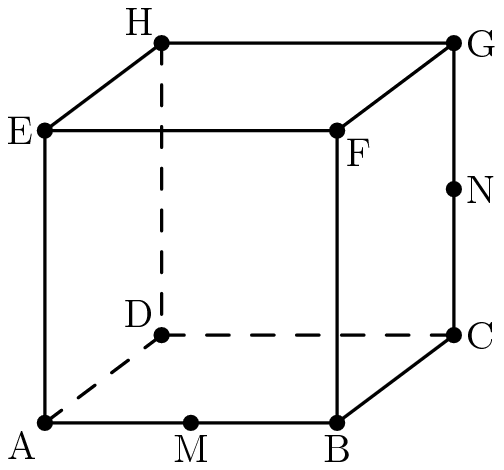
\includegraphics[width = 50.400000000000006mm]{img/fig0.png}
\end{center}